\documentclass[headings=standardclasses, headings=big]{scrreprt}

\usepackage{lmodern}
\usepackage{amssymb,amsmath}
\usepackage{ifxetex,ifluatex}
\usepackage{fixltx2e} % provides \textsubscript
\ifnum 0\ifxetex 1\fi\ifluatex 1\fi=0 % if pdftex
  \usepackage[T1]{fontenc}
  \usepackage[utf8]{inputenc}
\else % if luatex or xelatex
  \ifxetex
    \usepackage{mathspec}
  \else
    \usepackage{fontspec}
  \fi
  \defaultfontfeatures{Ligatures=TeX,Scale=MatchLowercase}
\fi
% use upquote if available, for straight quotes in verbatim environments
\IfFileExists{upquote.sty}{\usepackage{upquote}}{}
% use microtype if available
\IfFileExists{microtype.sty}{%
\usepackage[]{microtype}
\UseMicrotypeSet[protrusion]{basicmath} % disable protrusion for tt fonts
}{}
\PassOptionsToPackage{hyphens}{url} % url is loaded by hyperref
\usepackage[unicode=true]{hyperref}
\hypersetup{
            pdfborder={0 0 0},
            breaklinks=true}
\urlstyle{same}  % don't use monospace font for urls
\usepackage{longtable,booktabs}
% Fix footnotes in tables (requires footnote package)
\IfFileExists{footnote.sty}{\usepackage{footnote}\makesavenoteenv{long table}}{}
\usepackage{graphicx,grffile}
\makeatletter
\def\maxwidth{\ifdim\Gin@nat@width>\linewidth\linewidth\else\Gin@nat@width\fi}
\def\maxheight{\ifdim\Gin@nat@height>\textheight\textheight\else\Gin@nat@height\fi}
\makeatother
% Scale images if necessary, so that they will not overflow the page
% margins by default, and it is still possible to overwrite the defaults
% using explicit options in \includegraphics[width, height, ...]{}
\setkeys{Gin}{width=\maxwidth,height=\maxheight,keepaspectratio}
\IfFileExists{parskip.sty}{%
\usepackage{parskip}
}{% else
\setlength{\parindent}{0pt}
\setlength{\parskip}{6pt plus 2pt minus 1pt}
}
\setlength{\emergencystretch}{3em}  % prevent overfull lines
\providecommand{\tightlist}{%
  \setlength{\itemsep}{0pt}\setlength{\parskip}{0pt}}
\setcounter{secnumdepth}{0}
% Redefines (sub)paragraphs to behave more like sections
\ifx\paragraph\undefined\else
\let\oldparagraph\paragraph
\renewcommand{\paragraph}[1]{\oldparagraph{#1}\mbox{}}
\fi
\ifx\subparagraph\undefined\else
\let\oldsubparagraph\subparagraph
\renewcommand{\subparagraph}[1]{\oldsubparagraph{#1}\mbox{}}
\fi

% set default figure placement to htbp
\makeatletter
\def\fps@figure{htbp}
\makeatother



\usepackage[portuguese]{babel}
\usepackage[a4paper,tmargin=1cm]{geometry}

\usepackage{graphics}
\usepackage{listings}

\title{Sucuri}
\subtitle{Uma linguagem baseada em Python}
\author{João Paulo T. I. Z., Ranieri S. A., William K. A.}
\date{\today}

\begin{document}

\maketitle

\clearpage

\section{A linguagem}

A linguagem é planejada tendo como base algumas ideias de Python, Javascript e
Haskell. Para geração do analisador léxico, foi utilizada as ferramentas FLEX
(para especificação do léxico) e BISON (para gerar o código-fonte do
analisador).

Exemplo de código válido na linguagem Sucuri:

\lstinputlisting{../examples/geometry.scr}

\clearpage

\section{Especificação Léxica}

Inicialmente são definidas algumas regex de apoio:

\begin{verbatim}
D [0-9]                         % Reconhece dígitos

L [a-zA-Z_!@$?]                 % Reconhece qualquer símbolo
                                % possível em um identificador

NO_SQUOTE_STRING_LITERAL [^']*  % Qualquer _string literal_
                                % que não possua aspas simples

NO_DQUOTE_STRING_LITERAL [^"]*  % Qualquer _string literal_
                                % que não possua aspas duplas
\end{verbatim}

Além de duas funções, \texttt{count()}, que realiza contagem de colunas para
gerar uma melhor mensagem de erro (caso ocorra), e \texttt{indent\_level()},
que informa o nível de identação atual.

\subsection{Identificadores}

Identificadores são compostos por qualquer sequência de \texttt{L} ou
\texttt{D} não separados por espaços, podendo conter ``.'' (não no início, no
final nem sucedidos por dígitos).

\subsection{Literais}

\begin{minipage}{\textwidth}
São assumidos como literais de inteiros qualquer construção de somente dígitos:

\begin{verbatim}

# Inteiros válidos:

1
10
0
0000  % Tratado como 0
300
-10   % É reconhecido o "10" como literal inteiro e o "-" como operador unário
      % operado sobre o "10"

\end{verbatim}

Assim, sua \textit{regex} se torna \texttt{\{D\}+} (1 ou mais dígitos
consecutivos).
\end{minipage}

\begin{minipage}{\textwidth}
São assumidos como ponto-flutuante todo literal composto por números e que
tenha um ``.'' no início, meio ou fim do literal:

\begin{verbatim}

1   % Inteiro
1.  % Float
.1  % Float
-1. % "1." reconhecido como literal float, unário "-" operado em "1."

.   % Erro léxico

\end{verbatim}

Assim, sua \textit{regex} é separada em duas:

\begin{itemize}
    \item \texttt{"."\{D\}+} --- Reconhece \textit{floats} iniciados em ".";
    \item \texttt{\{D\}+"."\{D\}*} --- Reconhece \textit{floats} com "." no
        meio ou final;
\end{itemize}
\end{minipage}

\vspace{1em}

\begin{minipage}{\textwidth}
    \textit{String literals} são compostos de qualquer sequência de caracteres que:
    \begin{itemize}
        \item Estão entre aspas simples (') e não possuem outra aspa simples no
            meio (reconhecido pela \textit{regex}
            \texttt{"'"\{NO\_SQUOTE\_STRING\_LITERAL\}"'"}).
        \item Estão entre aspas dupla (") e não possuem outra aspa dupla no
            meio (reconhecido pela \textit{regex}
            \texttt{"\textbackslash\char`\""\{NO\_DQUOTE\_STRING\_LITERAL\}"\textbackslash\char`\""}).
    \end{itemize}
\end{minipage}

Operadores:

\begin{verbatim}
% Unários
not
-

% Comparativos
!=
=
<
<=
>
>=


% Matemáticos
+
-
*
**
/

% Lógicos
and
or
xor

% Outros
(
)

\end{verbatim}

Palavras reservadas:

\begin{verbatim}

% Estruturas de controle
class  % Define um novo tipo
if
else
for
while

% Retornos
return
throw

as     % Serve para alias
catch  % Captura exceções por throw
export % Define o elemento como público
from   % Para importação parcial de um módulo
import % Para importar um módulo
in     % Para iteração (for i in set)
let    % Definição
\end{verbatim}

Há também a definição de elipse (\texttt{...}) para parâmetros variádicos.

\clearpage

\section{Grafo de sintaxe e especificação EBNF}

\begin{minipage}{\textwidth}
    \protect\hypertarget{code}{}{code:}

    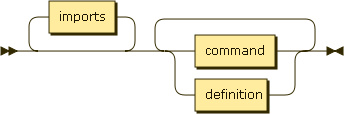
\includegraphics[width=5.18750in,height=1.00000in]{diagram/code.png}

    \begin{verbatim}
    code     ::= ( import_stmt NEWLINE )* ( stmt | definition )+
    \end{verbatim}

    no references

\end{minipage}

\begin{minipage}{\textwidth}
    \protect\hypertarget{atom}{}{atom:}

    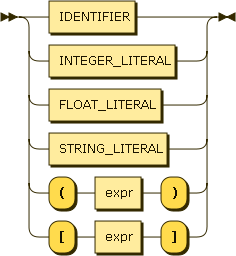
\includegraphics[width=2.45833in,height=2.66667in]{diagram/atom.png}

    \begin{verbatim}
    atom     ::= IDENTIFIER
           | INTEGER_LITERAL
           | FLOAT_LITERAL
           | STRING_LITERAL
           | '(' expr ')'
           | '[' expr ']'
    \end{verbatim}

    referenced by:

    \begin{itemize}
            \tightlist
        \item
            \protect\hyperlink{arglist}{arglist}
        \item
            \protect\hyperlink{assignment_expr}{assignment\_expr}
        \item
            \protect\hyperlink{atom_expr}{atom\_expr}
        \item
            \protect\hyperlink{function_params_list}{function\_params\_list}
    \end{itemize}

\end{minipage}

\begin{minipage}{\textwidth}
    \protect\hypertarget{atom_expr}{}{atom\_expr:}

    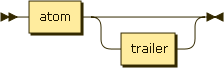
\includegraphics[width=2.33333in,height=0.70833in]{diagram/atom_expr.png}

    \begin{verbatim}
    atom_expr
         ::= atom trailer?
    \end{verbatim}

    referenced by:

    \begin{itemize}
            \tightlist
        \item
            \protect\hyperlink{unary_expr}{unary\_expr}
    \end{itemize}

\end{minipage}

\begin{minipage}{\textwidth}
    \protect\hypertarget{trailer}{}{trailer:}

    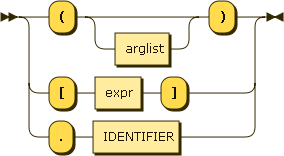
\includegraphics[width=2.95833in,height=1.62500in]{diagram/trailer.png}

    \begin{verbatim}
    trailer  ::= '(' arglist? ')'
           | '[' expr ']'
           | '.' IDENTIFIER
    \end{verbatim}

    referenced by:

    \begin{itemize}
            \tightlist
        \item
            \protect\hyperlink{atom_expr}{atom\_expr}
    \end{itemize}

\end{minipage}

\begin{minipage}{\textwidth}
    \protect\hypertarget{unary_expr}{}{unary\_expr:}

    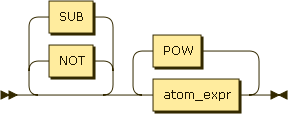
\includegraphics[width=3.00000in,height=1.18750in]{diagram/unary_expr.png}

    \begin{verbatim}
    unary_expr
         ::= ( NOT | SUB )* atom_expr ( POW atom_expr )*
    \end{verbatim}

    referenced by:

    \begin{itemize}
            \tightlist
        \item
            \protect\hyperlink{multiplicative_expr}{multiplicative\_expr}
    \end{itemize}

\end{minipage}

\begin{minipage}{\textwidth}
    \protect\hypertarget{multiplicative_expr}{}{multiplicative\_expr:}

    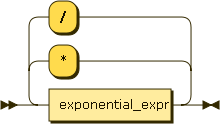
\includegraphics[width=1.93750in,height=1.29167in]{diagram/multiplicative_expr.png}

    \begin{verbatim}
    multiplicative_expr
         ::= unary_expr ( ( MUL | DIV ) unary_expr )*
    \end{verbatim}

    referenced by:

    \begin{itemize}
            \tightlist
        \item
            \protect\hyperlink{additive_expr}{additive\_expr}
    \end{itemize}

\end{minipage}

\begin{minipage}{\textwidth}
    \protect\hypertarget{additive_expr}{}{additive\_expr:}

    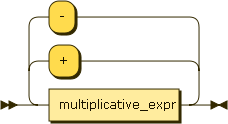
\includegraphics[width=2.37500in,height=1.29167in]{diagram/additive_expr.png}

    \begin{verbatim}
    additive_expr
         ::= multiplicative_expr ( ( ADD | SUB ) multiplicative_expr )*
    \end{verbatim}

    referenced by:

    \begin{itemize}
            \tightlist
        \item
            \protect\hyperlink{relational_expr}{relational\_expr}
    \end{itemize}

\end{minipage}

\begin{minipage}{\textwidth}
    \protect\hypertarget{relational_expr}{}{relational\_expr:}

    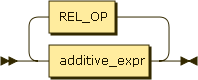
\includegraphics[width=2.06250in,height=2.20833in]{diagram/relational_expr.png}

    \begin{verbatim}
    relational_expr
         ::= additive_expr ( ( LT | LE | GT | GE ) additive_expr )*
    \end{verbatim}

    referenced by:

    \begin{itemize}
            \tightlist
        \item
            \protect\hyperlink{equality_expr}{equality\_expr}
    \end{itemize}

\end{minipage}

\begin{minipage}{\textwidth}
    \protect\hypertarget{equality_expr}{}{equality\_expr:}

    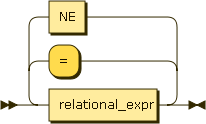
\includegraphics[width=2.14583in,height=1.29167in]{diagram/equality_expr.png}

    \begin{verbatim}
    equality_expr
         ::= relational_expr ( ( EQ | NE ) relational_expr )*
    \end{verbatim}

    referenced by:

    \begin{itemize}
            \tightlist
        \item
            \protect\hyperlink{expr}{expr}
    \end{itemize}

\end{minipage}

\begin{minipage}{\textwidth}
    \protect\hypertarget{expr}{}{expr:}

    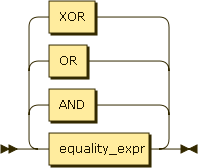
\includegraphics[width=2.06250in,height=1.75000in]{diagram/expr.png}

    \begin{verbatim}
    expr     ::= equality_expr ( ( AND | OR | XOR ) equality_expr )*
    \end{verbatim}

    referenced by:

    \begin{itemize}
            \tightlist
        \item
            \protect\hyperlink{atom}{atom}
        \item
            \protect\hyperlink{exprlist}{exprlist}
        \item
            \protect\hyperlink{for_stmt}{for\_stmt}
        \item
            \protect\hyperlink{if_stmt}{if\_stmt}
        \item
            \protect\hyperlink{stmt}{stmt}
        \item
            \protect\hyperlink{trailer}{trailer}
        \item
            \protect\hyperlink{while_stmt}{while\_stmt}
    \end{itemize}

\end{minipage}

\begin{minipage}{\textwidth}
    \protect\hypertarget{exprlist}{}{exprlist:}

    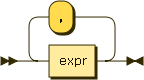
\includegraphics[width=1.50000in,height=0.83333in]{diagram/exprlist.png}

    \begin{verbatim}
    exprlist ::= expr ( ',' expr )*
    \end{verbatim}

    referenced by:

    \begin{itemize}
            \tightlist
        \item
            \protect\hyperlink{for_stmt}{for\_stmt}
        \item
            \protect\hyperlink{stmt}{stmt}
    \end{itemize}

\end{minipage}

\begin{minipage}{\textwidth}
    \protect\hypertarget{import_stmt}{}{import\_stmt:}

    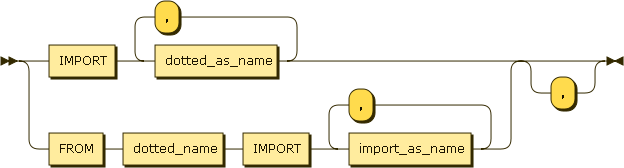
\includegraphics[width=6.50000in,height=1.75000in]{diagram/import_stmt.png}

    \begin{verbatim}
    import_stmt
         ::= ( IMPORT dotted_as_name ( ',' dotted_as_name )* | FROM dotted_name IMPORT import_as_name ( ',' import_as_name )* ) ','?
    \end{verbatim}

    referenced by:

    \begin{itemize}
            \tightlist
        \item
            \protect\hyperlink{code}{code}
    \end{itemize}

\end{minipage}

\begin{minipage}{\textwidth}
    \protect\hypertarget{dotted_as_name}{}{dotted\_as\_name:}

    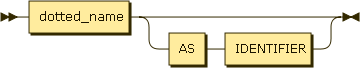
\includegraphics[width=3.75000in,height=0.70833in]{diagram/dotted_as_name.png}

    \begin{verbatim}
    dotted_as_name
         ::= dotted_name ( AS IDENTIFIER )?
    \end{verbatim}

    referenced by:

    \begin{itemize}
            \tightlist
        \item
            \protect\hyperlink{import_stmt}{import\_stmt}
    \end{itemize}

\end{minipage}

\begin{minipage}{\textwidth}
    \protect\hypertarget{import_as_name}{}{import\_as\_name:}

    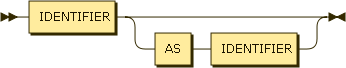
\includegraphics[width=3.60417in,height=0.70833in]{diagram/import_as_name.png}

    \begin{verbatim}
    import_as_name
         ::= IDENTIFIER ( AS IDENTIFIER )?
    \end{verbatim}

    referenced by:

    \begin{itemize}
            \tightlist
        \item
            \protect\hyperlink{import_stmt}{import\_stmt}
    \end{itemize}

\end{minipage}

\begin{minipage}{\textwidth}
    \protect\hypertarget{dotted_name}{}{dotted\_name:}

    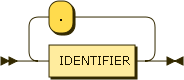
\includegraphics[width=1.91667in,height=0.83333in]{diagram/dotted_name.png}

    \begin{verbatim}
    dotted_name
         ::= IDENTIFIER ( '.' IDENTIFIER )*
    \end{verbatim}

    referenced by:

    \begin{itemize}
            \tightlist
        \item
            \protect\hyperlink{dotted_as_name}{dotted\_as\_name}
        \item
            \protect\hyperlink{import_stmt}{import\_stmt}
    \end{itemize}

\end{minipage}

\begin{minipage}{\textwidth}
    \protect\hypertarget{definition}{}{definition:}

    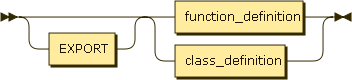
\includegraphics[width=3.66667in,height=0.83333in]{diagram/definition.png}

    \begin{verbatim}
    definition
         ::= EXPORT? ( function_definition | class_definition )
    \end{verbatim}

    referenced by:

    \begin{itemize}
            \tightlist
        \item
            \protect\hyperlink{code}{code}
    \end{itemize}

\end{minipage}

\begin{minipage}{\textwidth}
    \protect\hypertarget{function_definition}{}{function\_definition:}

    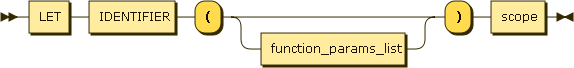
\includegraphics[width=5.97917in,height=0.70833in]{diagram/function_definition.png}

    \begin{verbatim}
    function_definition
         ::= LET IDENTIFIER '(' function_params_list? ')' scope
    \end{verbatim}

    referenced by:

    \begin{itemize}
            \tightlist
        \item
            \protect\hyperlink{class_scope}{class\_scope}
        \item
            \protect\hyperlink{definition}{definition}
    \end{itemize}

\end{minipage}

\begin{minipage}{\textwidth}
    \protect\hypertarget{function_params_list}{}{function\_params\_list:}

    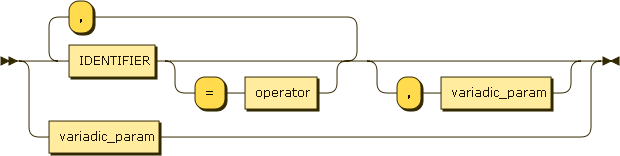
\includegraphics[width=6.31250in,height=1.62500in]{diagram/function_params_list.png}

    \begin{verbatim}
    function_params_list
         ::= IDENTIFIER ( EQ atom )? ( ',' IDENTIFIER ( EQ atom )? )* ( ',' variadic_param )?
           | variadic_param
    \end{verbatim}

    referenced by:

    \begin{itemize}
            \tightlist
        \item
            \protect\hyperlink{function_definition}{function\_definition}
    \end{itemize}

\end{minipage}

\begin{minipage}{\textwidth}
    \protect\hypertarget{variadic_param}{}{variadic\_param:}

    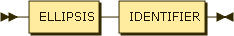
\includegraphics[width=2.43750in,height=0.37500in]{diagram/variadic_param.png}

    \begin{verbatim}
    variadic_param
         ::= ELLIPSIS IDENTIFIER
    \end{verbatim}

    referenced by:

    \begin{itemize}
            \tightlist
        \item
            \protect\hyperlink{function_params_list}{function\_params\_list}
    \end{itemize}

\end{minipage}

\begin{minipage}{\textwidth}
    \protect\hypertarget{scope}{}{scope:}

    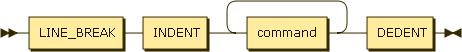
\includegraphics[width=5.25000in,height=0.54167in]{diagram/scope.png}

    \begin{verbatim}
    scope    ::= NEWLINE INDENT ( stmt NEWLINE )+ DEDENT
    \end{verbatim}

    referenced by:

    \begin{itemize}
            \tightlist
        \item
            \protect\hyperlink{for_stmt}{for\_stmt}
        \item
            \protect\hyperlink{function_definition}{function\_definition}
        \item
            \protect\hyperlink{if_stmt}{if\_stmt}
        \item
            \protect\hyperlink{while_stmt}{while\_stmt}
    \end{itemize}

\end{minipage}

\begin{minipage}{\textwidth}
    \protect\hypertarget{class_definition}{}{class\_definition:}

    
\includegraphics[width=3.47917in,height=0.37500in]{diagram/class_definition.png}

    \begin{verbatim}
    class_definition
         ::= CLASS IDENTIFIER class_scope
    \end{verbatim}

    referenced by:

    \begin{itemize}
            \tightlist
        \item
            \protect\hyperlink{definition}{definition}
    \end{itemize}

\end{minipage}

\begin{minipage}{\textwidth}
    \protect\hypertarget{class_scope}{}{class\_scope:}

    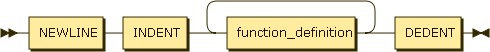
\includegraphics[width=5.10417in,height=0.54167in]{diagram/class_scope.png}

    \begin{verbatim}
    class_scope
         ::= NEWLINE INDENT function_definition+ DEDENT
    \end{verbatim}

    referenced by:

    \begin{itemize}
            \tightlist
        \item
            \protect\hyperlink{class_definition}{class\_definition}
    \end{itemize}

\end{minipage}

\begin{minipage}{\textwidth}
    \protect\hypertarget{stmt}{}{stmt:}

    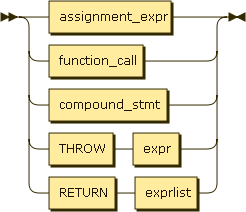
\includegraphics[width=2.56250in,height=2.20833in]{diagram/stmt.png}

    \begin{verbatim}
    stmt     ::= assignment_expr
           | function_call
           | compound_stmt
           | THROW expr
           | RETURN exprlist
    \end{verbatim}

    referenced by:

    \begin{itemize}
            \tightlist
        \item
            \protect\hyperlink{code}{code}
        \item
            \protect\hyperlink{scope}{scope}
    \end{itemize}

\end{minipage}

\begin{minipage}{\textwidth}
    \protect\hypertarget{assignment_expr}{}{assignment\_expr:}

    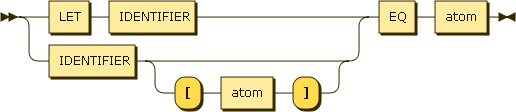
\includegraphics[width=5.37500in,height=1.16667in]{diagram/assignment_expr.png}

    \begin{verbatim}
    assignment_expr
         ::= ( LET IDENTIFIER | IDENTIFIER ( '[' atom ']' )? ) EQ atom
    \end{verbatim}

    referenced by:

    \begin{itemize}
            \tightlist
        \item
            \protect\hyperlink{stmt}{stmt}
    \end{itemize}

\end{minipage}

\begin{minipage}{\textwidth}
    \protect\hypertarget{function_call}{}{function\_call:}

    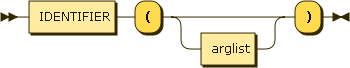
\includegraphics[width=3.64583in,height=0.70833in]{diagram/function_call.png}

    \begin{verbatim}
    function_call
         ::= IDENTIFIER '(' arglist? ')'
    \end{verbatim}

    referenced by:

    \begin{itemize}
            \tightlist
        \item
            \protect\hyperlink{stmt}{stmt}
    \end{itemize}

\end{minipage}

\begin{minipage}{\textwidth}
    \protect\hypertarget{arglist}{}{arglist:}

    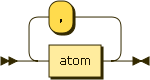
\includegraphics[width=1.56250in,height=0.83333in]{diagram/arglist.png}

    \begin{verbatim}
    arglist  ::= atom ( ',' atom )*
    \end{verbatim}

    referenced by:

    \begin{itemize}
            \tightlist
        \item
            \protect\hyperlink{function_call}{function\_call}
        \item
            \protect\hyperlink{trailer}{trailer}
    \end{itemize}

\end{minipage}

\begin{minipage}{\textwidth}
    \protect\hypertarget{compound_stmt}{}{compound\_stmt:}

    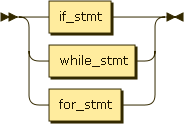
\includegraphics[width=1.91667in,height=1.29167in]{diagram/compound_stmt.png}

    \begin{verbatim}
    compound_stmt
         ::= if_stmt
           | while_stmt
           | for_stmt
    \end{verbatim}

    referenced by:

    \begin{itemize}
            \tightlist
        \item
            \protect\hyperlink{stmt}{stmt}
    \end{itemize}

\end{minipage}

\begin{minipage}{\textwidth}
    \protect\hypertarget{if_stmt}{}{if\_stmt:}

    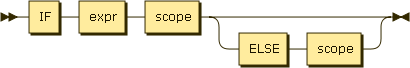
\includegraphics[width=4.27083in,height=0.70833in]{diagram/if_stmt.png}

    \begin{verbatim}
    if_stmt  ::= IF expr scope ( ELSE scope )?
    \end{verbatim}

    referenced by:

    \begin{itemize}
            \tightlist
        \item
            \protect\hyperlink{compound_stmt}{compound\_stmt}
    \end{itemize}

\end{minipage}

\begin{minipage}{\textwidth}
    \protect\hypertarget{while_stmt}{}{while\_stmt:}

    
\includegraphics[width=2.66667in,height=0.37500in]{diagram/while_stmt.png}

    \begin{verbatim}
    while_stmt
         ::= WHILE expr scope
    \end{verbatim}

    referenced by:

    \begin{itemize}
            \tightlist
        \item
            \protect\hyperlink{compound_stmt}{compound\_stmt}
    \end{itemize}

\end{minipage}

\begin{minipage}{\textwidth}
    \protect\hypertarget{for_stmt}{}{for\_stmt:}

    
\includegraphics[width=3.91667in,height=0.37500in]{diagram/for_stmt.png}

    \begin{verbatim}
    for_stmt ::= FOR exprlist IN expr scope
    \end{verbatim}

    referenced by:

    \begin{itemize}
            \tightlist
        \item
            \protect\hyperlink{compound_stmt}{compound\_stmt}
    \end{itemize}
\end{minipage}

\begin{center}\rule{0.5\linewidth}{\linethickness}\end{center}


\clearpage

\section{Arquivos}

Os arquivos FLEX e BISON são respectivamente \texttt{sucuri.l} e
\texttt{sucuri.y}. Exemplos de programas válidos se encontram na pasta
\texttt{examples/}. O código fonte do analisador é \texttt{sucuri.yy.c}.  Os
logs de saída aplicados no exemplo \texttt{examples/geometry.scr} estão no
arquivo \texttt{geometry-parse.ylog}.

\end{document}
